\chapter{Research Methodology}

Building upon the market overview and certification requirements discussed in the previous chapters, this chapter presents the technical methodology adopted to develop the Certification Tool. The tool is designed as a practical contribution to address the complexity of comparing FCR and aFRR prequalification requirements across European countries. The system is implemented as a containerised three-tier web application, consisting of an interactive Next.js frontend, a FastAPI backend and a PostgreSQL database, all orchestrated through Docker Compose. This chapter is divided into two major sections to describe the overall system architecture. The first segment demonstrates the architecture of the web app, including the frontend component design and the project structure, explaining how each technical layer supports the research objective. In the second segment, the architecture of the prequalification test setup is described, along with how technical requirements are significant within the whole system.

\section{Architecture of Certification Tool Web App}
The Certification Tool is designed as a component-driven, interactive web interface that translates complex certification requirements into a structured and user-friendly visualisation environment.

\subsection{User Interface Diagram}
\begin{figure}[htbp]
    \centering
    \IfFileExists{ui_diagram.png}{%
        
\includegraphics[width=0.8\textwidth]{ui_diagram.png}%
    }{%
        \IfFileExists{images/ui_diagram.png}{%
            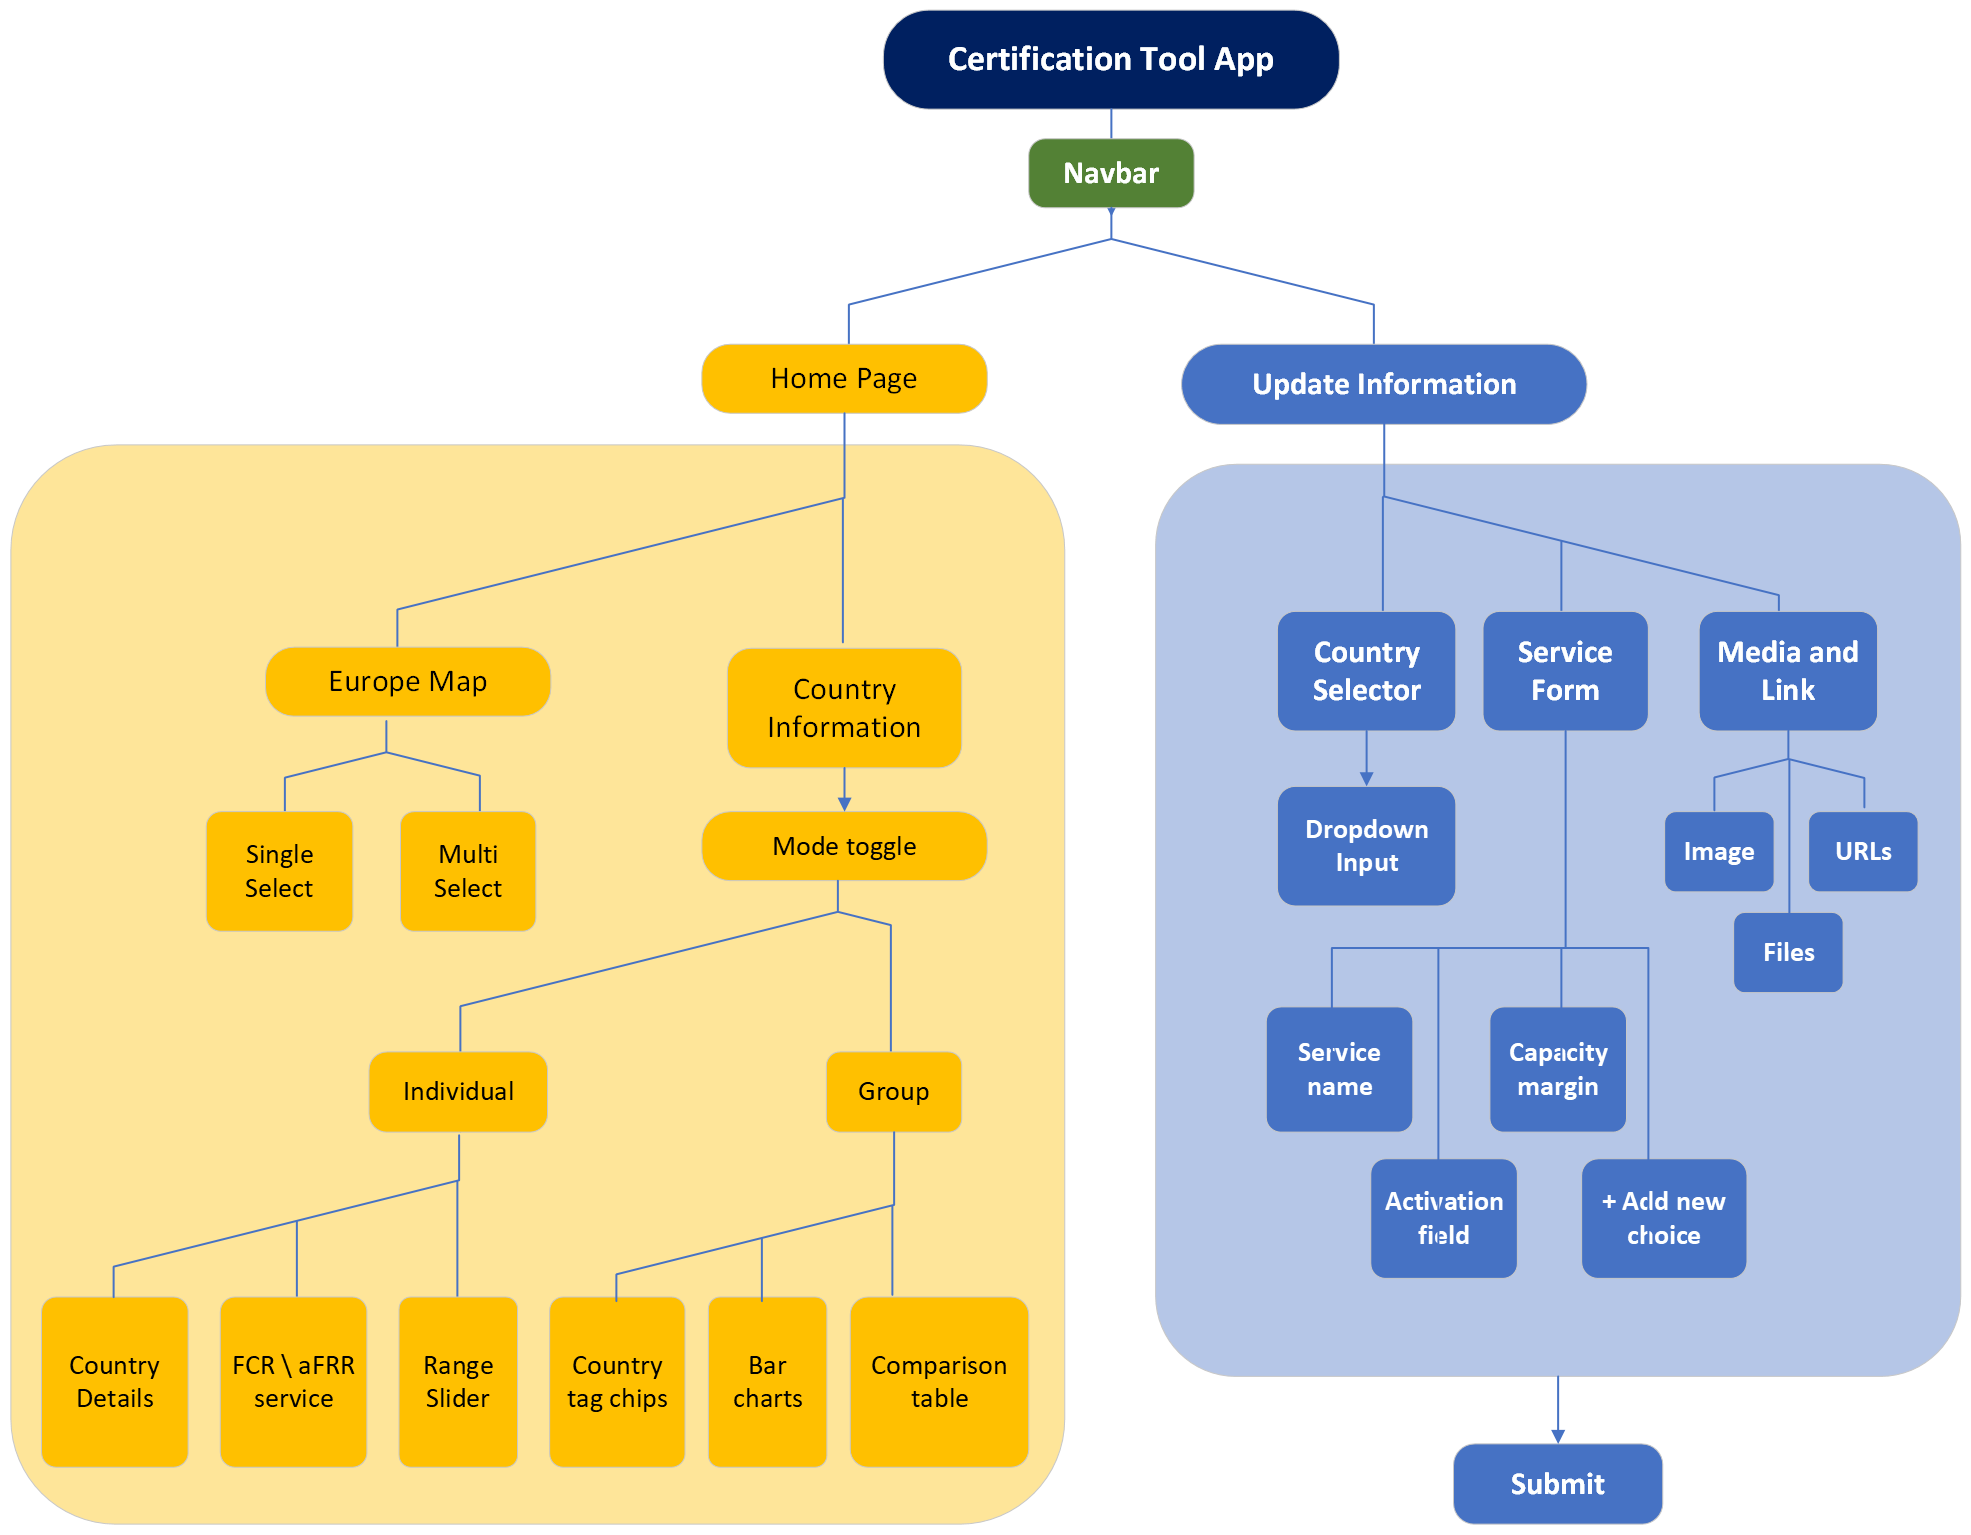
\includegraphics[width=0.8\textwidth]{images/ui_diagram.png}
        }{%
            \fbox{\parbox{0.75\textwidth}{\centering
            Image placeholder: add \texttt{ui\_diagram.png} either beside \texttt{main.tex} or inside an \texttt{images/} folder.}}
        }%
    }
    \caption{Diagram of Certification Tool web app}
    \label{fig:ui_diagram}
\end{figure}

This architecture is built on a modular design pattern and all UI elements are reusable and independent components. It makes the system more scalable and maintainable. This diagram briefly explains the overall structure of the web app, indicating the connections between the navigation and visual components.

\textbf{Navigation Layer:} The first part of the application is the navigation layer in the header component, which is organised with the name and navigation links of different pages. This section serves as the primary access point for two main functional areas of the application: the Home page and the Update Information page. The frontend is developed with the widely used Next.js framework for smooth transitions between route views without full page reloads. As a result, the user experience is enhanced by a clear distinction between the analytical functionalities of the Home page and the data management functionalities of the Update Information page.

\textbf{Home Page:} The Home page represents the main purpose of the application, consisting of visual effects and a comparison of certification requirements among various European countries. A responsive container holds the layout of the Certification Tool to ensure consistent alignment across different screen resolutions. The UI is divided into two sections: a European map-based component on the left side and a dynamic information panel on the right side. Both sections are logically dependent, because the map is dynamic and interactive, determining the content of the information panel in real time. This architecture is intended to provide a clear and quick overview of the technical requirements of active market participants.

\textbf{Switch Mode:} An important feature of the Home page is the toggle or mode-switching button, which allows users to analyse data in detail and in a comparative way. It controls a state variable and displays a rendered set of components. This function prevents navigation to separate pages and updates the system UI dynamically within the same view. Through this approach, interaction and maintenance of context become more efficient for users.

\textbf{Individual Mode:} In individual mode, the system displays all important criteria at the single-country level. Additionally, the interactive European map serves as the primary input component. This map is integrated into the system using a geospatial visualisation library within the React component structure. It is configured with a filtered geographic dataset to display only European countries. Each country is rendered as an interactive SVG element, allowing users to trigger events such as hover and click. This data is stored in the application state to propagate to other components.

The application state presents stored data in a dedicated panel, which is dynamically populated in the child component, following the working principle of the JavaScript framework. This information panel is further structured into service-specific views using the existing country dataset without reloading the component. Users can switch between Frequency Containment Reserve (FCR) and automatic Frequency Restoration Reserve (aFRR).

This subsection provides two types of data representation to indicate country-specific requirements. The first type is text-based, displayed with labels such as activation time and non-LER duration. The second type covers quantitative parameters such as capacity and error margin. Quantitative parameters are visualised using a custom static range slider component. The range slider is used to indicate minimum and maximum values and to enable a straightforward comparison between FCR and aFRR values. The complete UI is developed with smooth transitions to enhance user interaction.

\textbf{Group Mode:} This functionality comprises a comparison graph visualisation and a tabular format to support multiple countries for specific items. In this mode, the map supports multiple selections stored as a collection in the application state, allowing users to identify countries of interest and compare differences among them easily. Users can remove a selected country individually or clear all selections according to their preference.

The comparison view presents all data in either graphical or tabular form. Quantitative parameters are visualised using bar charts. Each bar within a normalised scale precisely indicates its limit, and different colours provide visual clarity across the page. This normalisation ensures clarity in the illustrative graph without distortion caused by extreme values. A React visualisation library named \textit{react-simple-map} in its offline version is applied to support dynamic data binding with real-time state updates when the selection changes. Simultaneously, the textual parameters are displayed in a structured fact table comprising precise numerical and categorical information to complement the visual effects. This dual representation enhances interpretability by combining intuitive visual insights with detailed data accuracy.

\textbf{Update Information:} The data management layer is introduced as the second part of the UI component architecture in the Update Information page. This part is designed to receive new data or update existing structured data from the user. The interface consists of multiple sections corresponding to the prequalification test requirements, each belonging to a specific category of certification parameters. The form begins with an auto-suggestion dropdown menu for the item ``Country''. Service-specific input fields then receive data for the available services of the selected country, such as FCR-D and FCR-N. These fields are grouped logically into activation time, capacity constraints, error margins and other operational requirements.

This form is designed to support multiple services for a country, allowing the user to update or remove services when new regulations are declared by the TSO. This is implemented using controlled form components and state arrays, enabling interface scalability. Additionally, the page supports the inclusion of supplementary resources, such as images, files and external links, to provide comprehensive data management.

In the final stage, data submission integrates the backend system with the frontend and a structured data format is transferred for permanent storage.

The UI architecture effectively transforms complex, document-style certification requirements into clear, interactive, structured data for business use. By integrating map-based selection, dynamic state management and multiple visualisation techniques, the Certification Tool becomes a well-structured platform for detailed and comparative analysis. The modular design ensures component independence, supporting future enhancements and integration with backend services.

\subsection{System Architecture}

\subsubsection{System Architecture Overview}
The Certification Tool is developed following a modern web-based system architecture consisting of a three-tier client-server model with a layered and modular design approach. Three primary components with different sets of rules and technologies form the complete system. These are the Frontend, Backend and Database. Each component interacts with the other components, and they communicate through pre-defined interfaces. The main purpose of the system architecture is to ensure maintainability, scalability and flexibility for future system enhancement or modification.

\begin{itemize}
    \item Frontend: This layer is known as the presentation layer. It handles user interaction and data visualisation. The presentation layer focuses on user experience and reduces the complexity of layout. This web app is built with Next.js.
    \item Backend: The backend is considered the application logic layer, which processes requests, manages business rules, coordinates data exchange between the frontend and the database, and provides security and data protection. The backend is developed with Python and the FastAPI framework.
    \item Database: The persistence layer is implemented using PostgreSQL to store different types of data in a structured format. It is deployed within a Docker container for quick development, portability and consistency without version conflicts.
\end{itemize}

Communication between the frontend and backend occurs via RESTful APIs over HTTP, while the backend interacts with the database using SQLAlchemy as an Object Relational Mapping (ORM) based access layer. As a result, the system maintains a clear separation between application logic and database operations.

\begin{figure}[htbp]
    \centering
    \IfFileExists{project_structure.png}{%
        
\includegraphics[width=1\textwidth]{project_structure.png}%
    }{%
        \IfFileExists{images/project_structure.png}{%
            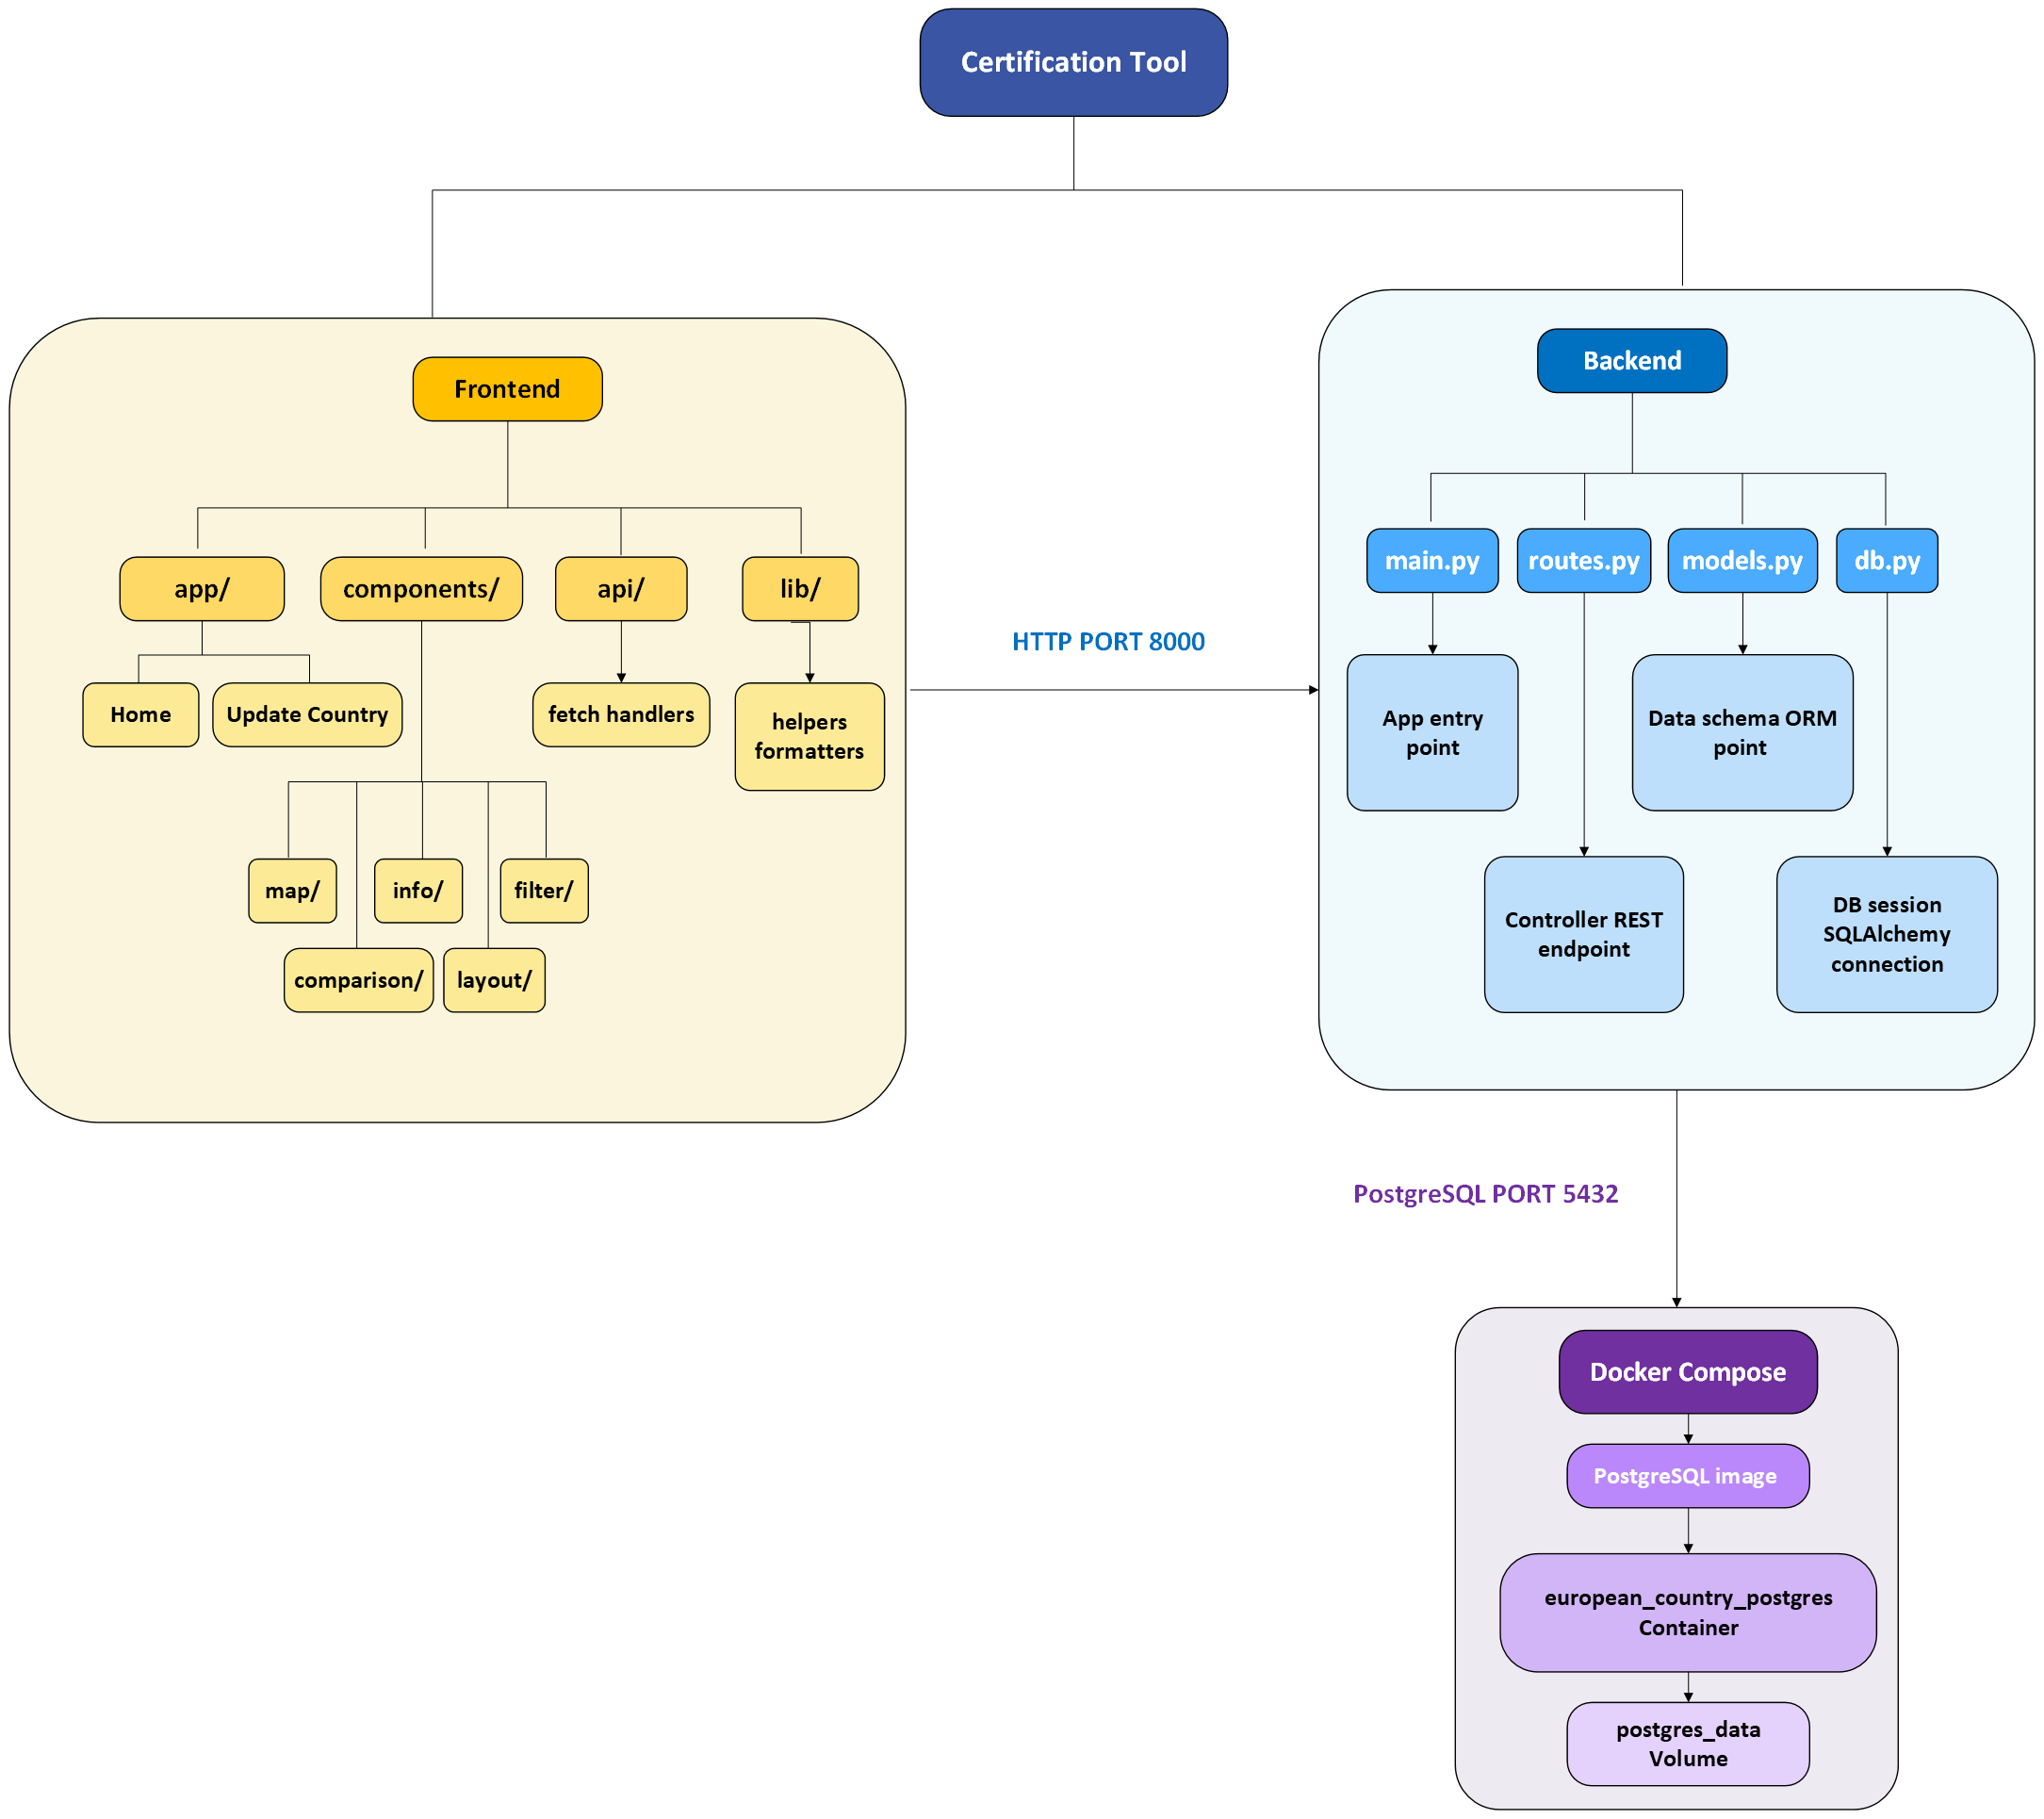
\includegraphics[width=1\textwidth]{images/project_structure.png}
        }{%
            \fbox{\parbox{0.75\textwidth}{\centering
            Image placeholder: add \texttt{project\_structure.png} either beside \texttt{main.tex} or inside an \texttt{images/} folder.}}
        }%
    }
    \caption{Diagram of system architecture}
    \label{fig:project_structure}
\end{figure}


\subsubsection{Architectural Style}
The client-server architectural style is adopted for the frontend and backend, which are decoupled and communicate via HTTP requests. Although each component is internally connected, the design allows for independent development and deployment while ensuring scalability and maintainability.

The backend utilises a layered architecture. It separates responsibilities into routing (controller layer), business logic and data access. This layered design reduces the complexity of debugging and testing, supports modularity, and enables future extension of the system.

In contrast, the frontend follows a component-based architecture to enhance UI performance. It is divided into reusable components such as map visualisation, country information panels and a comparison view. This design provides a compact solution for efficiency and reusability.


\subsubsection{Backend Architecture}
The backend follows a modular monolithic architecture pattern, with FastAPI selected for development. Although deployed as a single application, it is structured into multiple modules where each component is responsible for a specific functionality.

The entry point of the application initialises the FastAPI instance, verifies and validates middleware configuration such as Cross-Origin Resource Sharing (CORS), and registers API routes. This configuration enables secure communication between the frontend (running on port 3000) and the backend service.

A significant module named \textit{routes} defines the REST API endpoints for managing user requests. The purpose of these endpoints is to act as controllers, receiving HTTP requests, validating input data and returning structured JSON responses. The system supports operations such as retrieving country data, inserting new certification information and updating previously stored data in the database.

The final stage is the database connection layer, which manages communication with PostgreSQL. This layer has specific responsibilities such as loading configuration from environment variables, initialising the SQLAlchemy engine and providing session management for executing queries. Ultimately, the system becomes more consistent and gains robustness in database operations.


\subsubsection{Database and Containerisation}
For this application, a relational database called PostgreSQL is used for storing certification data. PostgreSQL is chosen due to its reliability, support for structured and semi-structured data, and its compatibility with SQLAlchemy.

The database is deployed using Docker and managed through a Docker Compose configuration. The PostgreSQL service runs inside a container, which is exposed on port 5432 and defined in the docker-compose.yml file. It allows the backend application to connect using a defined connection string. Docker ensures consistency for software development and deployment, and resolves configuration-related issues in the database environment.

Although SQLAlchemy is not a database system itself, it provides an ORM layer used by the backend to interact with PostgreSQL. The PostgreSQL port facilitates actual database communication, while SQLAlchemy provides an abstraction layer for query execution and schema definition.

\subsubsection{Frontend Architecture}
A modular structure following modern web development practices is implemented using Next.js and TypeScript. The frontend of the Certification Tool is organised into directories such as \textit{app}, \textit{components}, \textit{api} and \textit{lib}, each serving a distinct purpose.

The \textit{app} directory defines page-level routing to integrate the Home page and Update Info page within the same module. The Home page renders the Europe map, country information panel and comparison components. The Update Info page provides a form-based interface for inserting and modifying the technical requirements of certification data.

The \textit{components} directory introduces reusable UI modules categorised by functionality. It contains five components serving different purposes, named \textit{map}, \textit{info}, \textit{filter}, \textit{comparison} and \textit{layout}. The map component renders a user-friendly Europe map supporting both single and multi-country selection. The info component displays detailed data used for the prequalification test among selected countries. Both textual values and visual elements such as range sliders are combined in the component view. The comparison component enables group-level analysis, presenting data through various graphs and tabular formats.

For API communication and data transformation, the frontend includes utility modules. These utilities process backend responses and convert data into formats suitable for visualisation. For instance, they map textual constraints into numerical ranges.

\subsubsection{System Interaction Flow}
The system workflow operates through a structured interaction among the frontend, backend and database layers. A user interacts with the frontend by selecting countries on the map, or by submitting or modifying data. After this step, the application determines whether backend communication is required.

During data retrieval or modification, the frontend sends an HTTP request to the backend API. The backend processes the request through the routing layer and applies the necessary logic to interact with the database via SQLAlchemy sessions. The queries are executed in the database following SQL language rules and the generated result is returned to the backend for further processing. The result is then sent in standard JSON format to the frontend as a response to the end user.

The user interface updates the received data dynamically for each request. This final stage is the view layer, which handles displaying country-specific prequalification test criteria details, updating comparison charts and reflecting newly inserted data.

The Certification Tool represents a well-structured architecture that effectively manages and visualises prequalification test technical requirements. This section has explained the working process of the component-based frontend design, which enables user interaction through map-based selection, information panels with text and range sliders, and comparative visualisations of requirements published by TSOs. As a result, the tool achieves important goals such as modularity and scalability through a standard architecture. At the system level, the three-tier client-server architecture provides a clear separation among the presentation layer, application logic and data persistence mechanism, through the use of Next.js, FastAPI and PostgreSQL. To enhance flexibility, maintainability and consistency, a modular backend structure and a containerised database are integrated. Ultimately, this architecture generates a scalable and reliable foundation that makes the analysis more efficient than a general solution, while supporting the comparison and maintenance of essential data across multiple European countries that actively participate in the electricity market.


\section{Architecture of Prequalification Test Setup}

\subsection{Architecture of Elia: Belgium}

\textbf{Activation Time \& Speed:} This criterion is the first step of verification of whether a BSP is eligible for certification. According to Elia, activation time and activation speed are used for different purposes but both describe how a unit reacts to a frequency deviation.

Activation time refers to the deadline, a specific time-based milestone by which a unit must deliver certain percentages of its FCR capacity. There are two different scenarios for the activation time: Real-Time Delivery and the Prequalification Test.

\noindent 1. Real Delivery to Grid: This is the actual event of service delivery to the grid. It has three time limits.
\begin{itemize}
    \item Initial Activation Time: This is the first time limit to start a response following a frequency deviation. According to Elia, the time limit is 2 seconds after the frequency deviation has started.
    \item Half Activation Time: This is the second time limit to deliver at least 50\% of the target capacity. For instance, a BSP must deliver at least 0.5~MW of capacity within 15 seconds if they bid for 1~MW.
    \item Full Activation Time: The final time limit to deliver full capacity is at most 30 seconds from the start of the frequency deviation.
\end{itemize}
2. Prequalification Test: The prequalification test setup requires an extra 5 seconds for technical tolerance in the test environment. The frequency deviation does not occur smoothly during the test; instead, it deviates in 50~mHz steps as a ramp. The main differences are described below.
\begin{itemize}
    \item 50~mHz frequency deviation step: The response will be proportional to the frequency deviation. The time limit is 12.5 seconds (7.5~sec + 5~sec), where 7.5 seconds is the required activation time (derived from the proportional 30-second global rule) and 5 seconds is for system lag tolerance.
    \item Stability Constraint: After completing the first step, the BSP must maintain at least 90\% of that volume for 2 minutes before moving to the next step.
\end{itemize}
These rules apply for each 50~mHz frequency deviation step until the end of the test.

In contrast, activation speed indicates the behaviour of the power response. It refers to the linearity or ramping rate by which a BSP determines how the expected volume will be delivered by the deadline.

\textbf{Capacity:} This data has several constraints that must be followed by the BSP. These are:
\begin{itemize}
    \item Minimum Bid Size: The minimum volume for an FCR capacity bid is 1~MW.
    \item Bid Resolution: Bids must be submitted in increments of 1~MW, meaning the bid must be a whole number.
    \item Aggregation for Small Assets: A group of small units each with less than 1~MW capacity can be aggregated to reach at least 1~MW.
    \item Indivisible Maximum Bid: The maximum bid size is 25~MW and cannot be partially accepted.
    \item Maximum Portfolio Limit: This value will be determined by the result of the prequalification test.
    \item Virtual Delivery Point: The capacity of a Virtual Delivery Point must be less than 1.5~MW.
\end{itemize}


\subsection{Architecture of APG: Austria}
The Austrian Power Grid (APG) provides the opportunity to bid for ancillary services under different names. These are the Primary Control Reserve Service, Secondary Control Reserve Service, and Tertiary Control Reserve Service. Here, the Primary Control Reserve Service follows similar rules to FCR, the Secondary Control Reserve Service follows aFRR, and the Tertiary Control Reserve Service follows mFRR. In this section, all requirements and the system architecture refer to the Primary Control Reserve Service.

\textbf{Activation Time:} This criterion covers the time limits for 50\% and 100\% reserve activation following the start of a frequency deviation.
\begin{itemize}
    \item 50\% Activation: The primary control power must be at least half-activated within 15 seconds. [Resource: \texttt{PRR\_PQ\_23\_05\_2014\_Formular.pdf}, page: 9, sec: 3.1.10]
    \item 100\% Activation: The primary control power must be fully activated within 30 seconds. [Resource: \texttt{PRR\_PQ\_23\_05\_2014\_Formular.pdf}, page: 9, sec: 3.1.10]
\end{itemize}
\textbf{Capacity Requirement:} The capacity requirement defines the minimum and maximum limits of power that the asset must supply or consume. The capacity limit can be defined with or without a delivery type, such as symmetric, asymmetric or both. According to APG, all control services are required to specify a delivery type.
\begin{itemize}
    \item Minimum Capacity: The control range of an applicant's reserve group must be at least $\pm 1$~MW [Resource: \texttt{PRR\_PQ\_23\_05\_2014\_Formular.pdf}, page: 8, sec: 3.1.6]. This delivery must be symmetric; no asymmetric delivery is permitted [Resource: \texttt{Erläuterungen\_Präqualifikation\_20150910.pdf}, page: 5, sec: 2.1].
    \item Maximum Capacity: This value depends on the prequalified capacity. [Resource: Primärregelung (PRR) - website]
    \item Maximum Indivisible Bid: The maximum bid size is $\pm 25$~MW, which can be either fully accepted or completely rejected. [Resource: Primärregelung (PRR) - website]
    \item Resolution: The bid resolution is 1~MW and bids can be submitted in whole MW increments. [Resource: Primärregelung (PRR) - website]
\end{itemize}
\textbf{Delivery Duration:} To verify the stability and robustness of assets, delivery duration is an essential parameter. There are 2 scenarios for checking the maximum sustained activation.
\begin{itemize}
    \item Large frequency deviation: The BSP must continue full activation for at least 30 minutes without interruption for a frequency deviation of $\pm 200$~mHz. [Resource: \texttt{PRR\_PQ\_23\_05\_2014\_Formular.pdf}, page: 10, sec: 3.1.14]
    \item Small frequency deviation: For a frequency deviation of less than $\pm 200$~mHz, the asset will be partially activated rather than fully activated, and this must be sustained for longer than 30 minutes. For instance, a $\pm 100$~mHz frequency deviation requires around 50\% activation for approximately 60 minutes. [Resource: \texttt{PRR\_PQ\_23\_05\_2014\_Formular.pdf}, page: 10, sec: 3.1.14]
\end{itemize}
\textbf{Non-LER Duration:} The Limited Energy Reservoir (LER) is the most important prerequisite for validating the stability and robustness of an asset across moderate to extreme scenarios. Compared with other TSOs, APG classifies asset types differently. All batteries are counted in the LER group, while power plants such as gas, hydro and generator units fall into the non-LER group, as smaller technical units may be unable to generate power continuously and may face resource scarcity within a few hours. No specific time limit is defined for this criterion in the available resources [Resource: \texttt{Erläuterungen\_Präqualifikation\_20150910.pdf}, page: 17, sec: 10].

\textbf{Meter Accuracy:} Meter accuracy can be assessed in two ways: as a minimum measurement accuracy or as a maximum measurement error. For APG, the maximum frequency measurement error is $\pm 5$~mHz [Resource: \texttt{PRR\_PQ\_23\_05\_2014\_Formular.pdf}, page: 8, sec: 3.1.8].

\textbf{Error Margin:} This criterion has no specific rule defining the limits of over-delivery and under-delivery for either upward or downward regulation.

\textbf{Controller:} The information regarding the controller is not straightforward; it relates more to equipment setup rules within the transmission system. The primary control response must be local and present at each technical unit. The frequency meter and the controller must be physically located at the technical unit. The response cannot depend on any remote signal, cloud platform or internet connection. According to the Austrian TSO:
\begin{itemize}
    \item Internet-based solutions are explicitly excluded. [Resource: \texttt{PRR\_Annex\_Infomationstechnik.pdf}, page: 3--4, sec: 1.1.3]
    \item The 30-second maximum activation time is too tight to accommodate round-trip latency to a remote or cloud-based controller.
\end{itemize}
Furthermore, the prequalification documentation refers to a primary controller or turbine controller in power plants, which is a physical device installed directly on a generating unit. It automatically adjusts the turbine's mechanical power output in response to detected frequency deviations. [Resource: \texttt{primaerregelung 1st FAQ} - online]

\textbf{Sampling Time:} The sampling time is 2 seconds, which applies to both the archived data resolution and the online data transmission cycle to APG. [Resource: \texttt{PRR\_PQ\_23\_05\_2014\_Formular.pdf}, page: 12, sec: 3.2.4, 3.2.5]

\textbf{Regulation Type:} For primary control reserve, only the symmetric type is permitted. [Resource: \texttt{Erläuterungen\_Präqualifikation\_20150910.pdf}, page: 5, sec: 2.1]

\textbf{Time Window:} The entire primary control reserve must be available without interruption within any one of the 6 daily product blocks, each covering a 4-hour window. [Resource: \texttt{primaerregelung} - online]
